\chapter{Desarrollo}

El sistema IoT propuesto para una habitación de un entorno Smart House representado por el esquema de la Figura \ref{fig:diagramas}, pretende ser fácil de visualizar y manipular por el usuario, por este motivo se desarrolla una aplicación web (software) que permite la cómoda navegación a través de ella y que las interacciones humano-máquina sean de manera intuitiva. Esta característica del sistema está diseñada de tal manera que solo los usuarios puedan ver el estado de la habitación, ya que para hacerlo es necesario ingresar las credenciales oficiales otorgadas por el Usuario Administrador, el cual es uno de los tres roles de usuario existentes en el sistema, junto con el rol de Usuario Casa y Usuario Habitación.\\

Como se mencionó anteriormente, el Usuario Administrador es quien otorga las credenciales a los demás usuarios, ya que este tiene la facultad de crear, editar y eliminar los registros de la aplicación, lo cual a su vez lo hace exclusivo, es decir, no esta abierto para el público o los clientes.\\ 

En ese orden de ideas, los demás usuarios tienen privilegios limitados a las necesidades de cada rol, es decir, los Usuarios Casa tienen acceso a la revisión y edición de algunos campos de las viviendas registradas a su nombre y de los usuarios Habitación vinculados a él, además de poder gestionar los dispositivos en el hogar. Cabe resaltar que este usuario es opcional, puesto que un Usuario Habitación puede operar de manera independiente, teniendo esta la simple vista de los dispositivos conectados, es decir, tiene acceso a el panel de control que representa la habitación en cuestión.\\
 
La aplicación web está conectada con la tarjeta Smart House (Hardware), ya que esta cuenta con conexión a Internet vía WiFi, la cual es gestionada por el Firmware del dispositivo, con el fin de realizar el vínculo entre software y hardware de manera adecuada. Además, el firmware gestiona las múltiples tareas que realiza la tarjeta, como lo son la lectura de datos y la gestión de las cargas conectadas a las diferentes salidas AC o DC, entre otras funcionalidades.\\

\begin{figure}[H]
	\centering
	\caption[Esquema del sistema IoT.]{Esquema del sistema IoT. [Imagen Propia]}
	\label{fig:diagramas}
	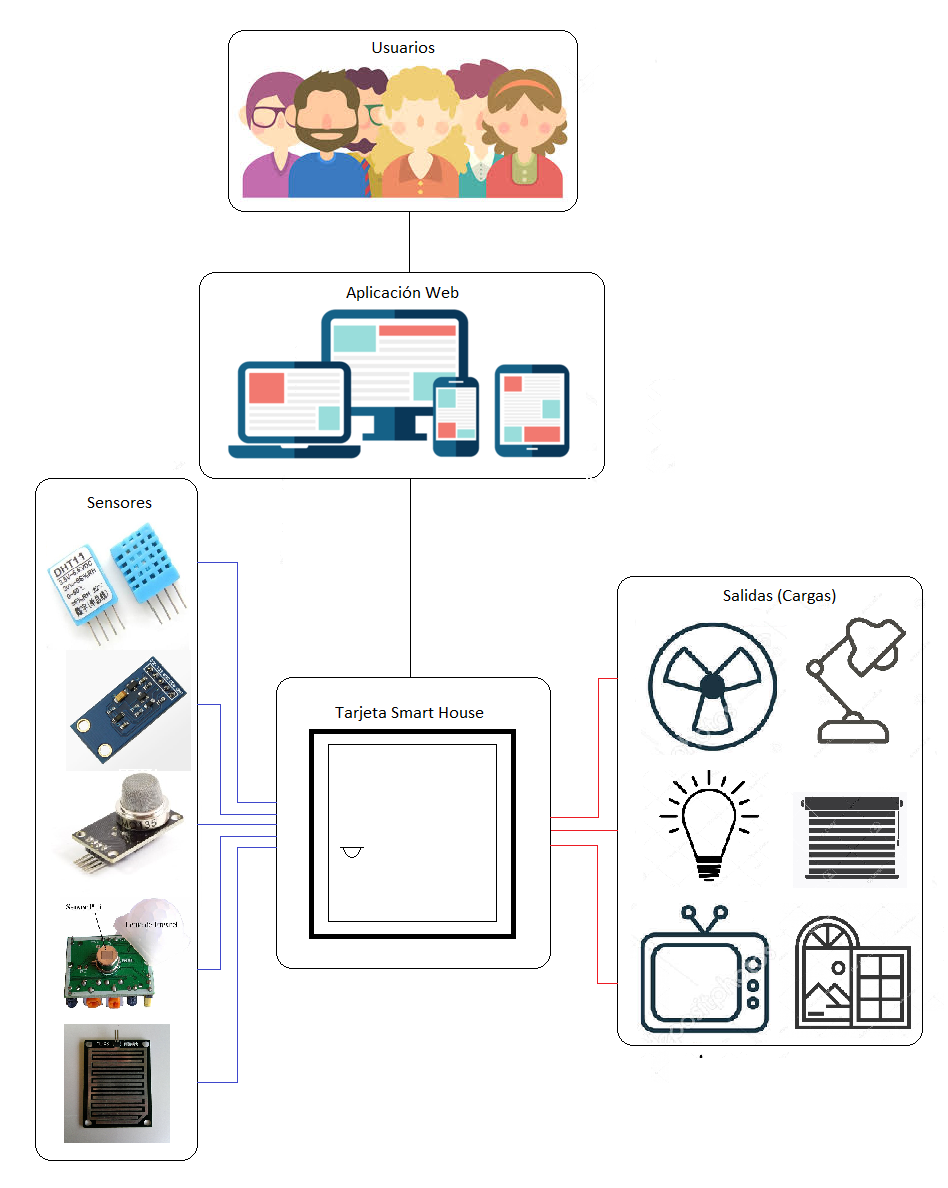
\includegraphics[width=0.7\linewidth]{Imagenes/Diagramas}
\end{figure}

Para la construcción del hardware se tomaron como referencia valores de operación presentes en el mercado, de modo que las salidas para cargas DC fueron definidas a un voltaje de 12V, ya que se comercializan dispositivos como lámparas LEDs o mecanismos capaces de abrir y cerrar ventanas o persianas con este nivel de tensión, entre otros. Por otra parte, el voltaje para las cargas AC se define con base en la red eléctrica doméstica de Colombia, siendo esta 110VAC. Para las entradas del dispositivo se cuenta con los sensores mencionados anteriormente en la Sección \ref{sec:sensors}, los cuales funcionan con voltajes lógicos de 5V y 3.3V. Estos sensores se eligen por ser los más usados en dicho ámbito además de que se acomodan a las necesidades de una habitación, como sensar presencia, temperatura, calidad del aire y demás.\\

Además, para el funcionamiento de la aplicación y el hardware se hace uso del ESP32 como unidad central de mando, ya que cuenta con un procesador de 32 bits de dos núcleos, de los cuales uno de ellos se encarga de la conexión WiFi, mientras que el otro se encarga de los demás procesos del sistema descritos en el presente capítulo. Adicionalmente, el ESP32 cuenta con múltiples salidas y entradas como DACs y ADCs, lo cual permite manejar salidas de audio, entradas analógicas y demás; las cuales se programan a través del framework oficial del ESP32, el ESP-IDF. La ventaja del ESP32 es su integración del WiFi, Bluetooth y otras capacidades en un solo chip en comparación con las distintas tarjetas presentes en el mercado; también su precio con respecto a las funcionalidades que este ofrece.\\

\section{Hardware}\label{sec:hw}

El diseño de hardware parte desde un concepto general de la solución, es decir, su estructura ilustrada en la Figura \ref{fig:tar}, está definida con el fin de abarcar de manera completa cada una de las funcionalidades necesarias para la correcta operación del dispositivo, a la vez que contempla características clave para cumplir con los objetivos propuestos, tales como las etapas de adquisición de datos encargada de recolectar la información del entorno de aplicación, etapa de control de cargas para manipular mecanismos como motores o dispositivos de iluminación, entre otras, de tal manera que al desarrollar cada etapa por separado, se logra crear el prototipo completo.\\

\begin{figure}[H]
	\centering
	\caption[Diagrama de la tarjeta Smart House.]{Diagrama de la tarjeta Smart House.  [Imagen Propia]}
	\label{fig:tar}
	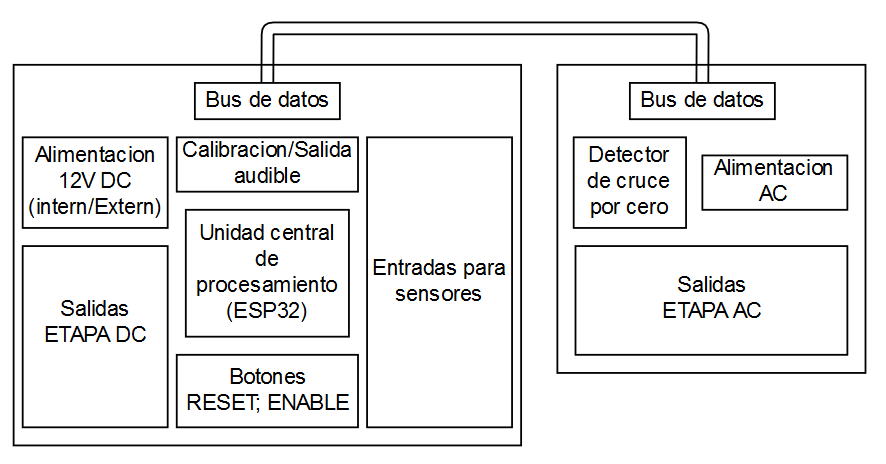
\includegraphics[width=0.7\linewidth]{Imagenes/Tarjeta}
\end{figure}

En primer lugar, al definir el ESP32 como unidad central de mando se tiene disponibilidad de 34 GPIO programables, entre los cuales algunos de ellos cuentan con diferentes enfoques más específicos como DAC y ADC, entre otros, los cuales son distribuidos para la adquisición de datos por parte de sensores, así como también la manipulación de las correspondientes cargas y demás salidas del dispositivo. Debido a que el ESP32 opera a un nivel lógico de 3.3V, se hace necesario garantizar este voltaje en algunas etapas de la estructura del hardware.\\

En la Tabla \ref{fig:tar}, se observan las características definidas para el diseño del hardware, basados en las cualidades y numero de pines con los cuales cuenta el ESP32 como limitante.\\


\begin{table}[H]
	\begin{center}
		\caption{Características Hardware.}
		\label{table:carac}
		\begin{tabular}{|c|c|c|}
			\hline 
			\textbf{Características Tarjeta SH} & \textbf{Cualidad/Cantidad} & \textbf{Métrica} \\ 
			\hline 
			Unidad central de mando & ESP32 & 1\\ 
			\hline 
			Entrada Sensores & 7 & 5VDC; 3.3VDC\\
			\hline 
			I2C & Si & 1\\
			\hline 
			Salidas/Cargas DC & 4 & 12VDC\\
			\hline 
			Salidas/Cargas AC & 6 & 110VAC\\
			\hline 
			Salida Audible & Si & 1\\
			\hline 
			WiFi & Si & 1\\ 
			\hline 
			Fuente Interna & 1 & 12VDC-2A\\
			\hline
			Conector Fuente Externa & 1 & 12VDC-5A Máx.\\
			\hline
		\end{tabular} 
	\end{center}
\end{table}

Con las características de operación definidas para el prototipo, y con ayuda del software Proteus se realizan simulaciones de algunas etapas del hardware, de tal manera que sea en menor cantidad las pruebas realizadas en protoboard antes de la implementación del prototipo, el cual fue diseñado en este software desde el esquemático hasta la placa de circuito impreso (PCB). En la Figura \ref{fig:esp32} se observa el diagrama esquemático de la tarjeta ESP32 construido junto con su distribución de pines, además de sus conexiones correspondientes dentro de este programa. El prototipo está separado en dos secciones, la etapa de potencia AC y la etapa DC, en la última, se encuentra la mayor parte de circuitos que funcionan con corriente directa.\\

\begin{figure}[H]
	\centering
	\caption[ESP32 creado en proteus.]{ESP32 creado en proteus. [Imagen Propia]}
	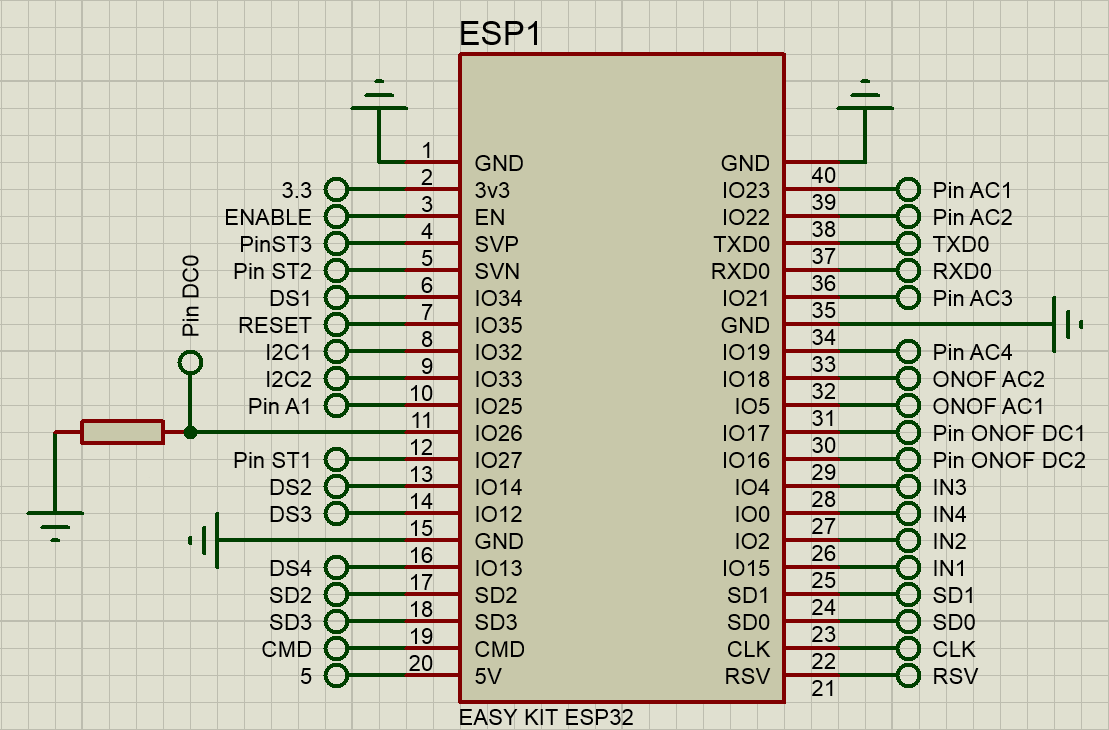
\includegraphics[width=0.5\linewidth]{Imagenes/ESP32}	
	\label{fig:esp32}
\end{figure}

	\subsection{Alimentación}
	
	En la Figura \ref{fig:balidc}\textbf{(a)} y \ref{fig:balidc}\textbf{(b)} se observa como está planteada la etapa de alimentación tanto para la etapa AC como la etapa DC respectivamente, la cual da soporte al funcionamiento total del dispositivo, es decir, se encarga de recibir la energía eléctrica y acondicionarla para dar correcto suministro a las diferentes etapas del hardware, incluyendo la unidad central de mando y los circuitos de control.\\
	
	Debido a que el voltaje DC más alto presenta una magnitud de 12V, se decide tomar este voltaje y reducirlo a los niveles lógicos requeridos para el manejo adecuado de dispositivos como sensores, así como también el ESP32. \\
	
	\begin{figure}[H]
		\centering
		\caption[Etapa de alimentacion AC y DC.]{Etapa de alimentacion AC y DC. [Imagen Propia]}
		\subfigure[Etapa Alimentación AC]{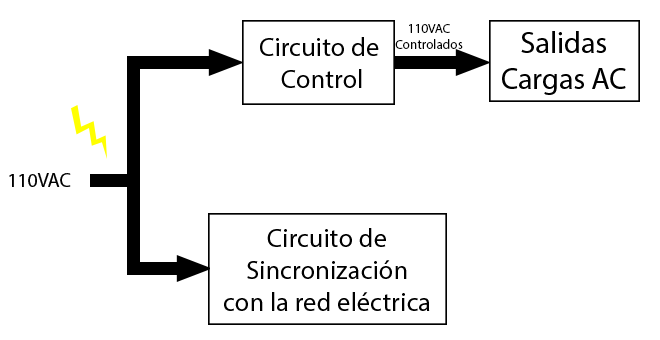
\includegraphics[width=0.5\linewidth]{Imagenes/B_AliAC}}
		\subfigure[Etapa Alimentación DC]{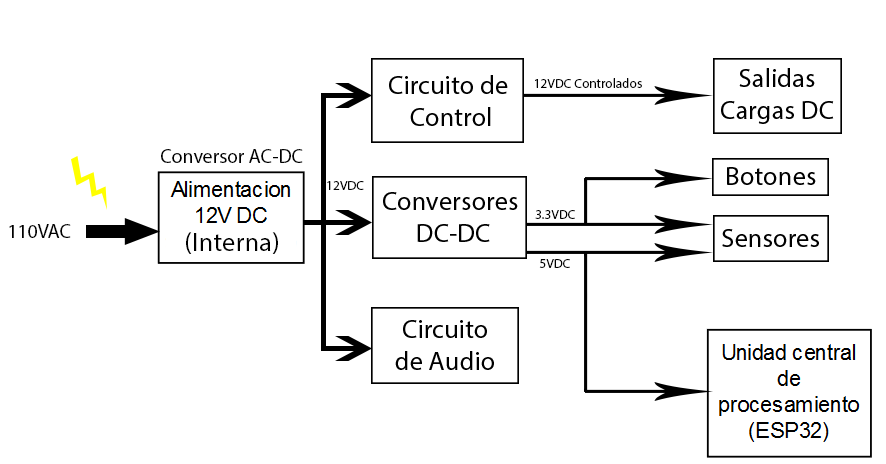
\includegraphics[width=0.6\linewidth]{Imagenes/B_Alimentacion}}
		\label{fig:balidc}
	\end{figure}
	
	
	\paragraph{Corriente alterna (AC):}
		El prototipo recibe el voltaje directamente de la red eléctrica a la que se encuentra conectado el entorno de aplicación, el cual está pensado para una habitación dentro de una Smart House; en el caso de Colombia, la red doméstica comúnmente otorga 110V AC, los cuales son regulados para el funcionamiento adecuado del prototipo, como la etapa de potencia AC y el detector de cruce por cero con el fin de sincronizar la tarjeta a dicha red eléctrica.\\
		
	\paragraph{Corriente directa (DC):}
		Para la alimentación DC del circuito, se hace uso de un conversor AC-DC que regula el voltaje de la red eléctrica a 12V DC, con los cuales se maneja la etapa de potencia DC, además de ser usados por dos módulos conversores DC-DC, mostrados en la Figura \ref{fig:DCDC}, ambos con entradas de 12V DC y con salidas a los niveles lógicos comunes, 5V y 3.3V, empleados con el fin de alimentar dispositivos como optoacopladores, transistores BJT o relevadores con activación de 5V, así como también la tarjeta de prototipo ESP32.\\
		
		Cabe resaltar que la tarjeta cuenta con una fuente interna de 12VDC a 2A para la etapa DC y una ranura para agregar una fuente externa de 12VDC a 5A si se desean controlar cargas a un máximo de 50W, en el Anexo C se encuentra como conmutar entre la fuente interna y externa.\\
			
		\begin{figure}[H]
			\centering
			\caption[Módulo conversor DC-DC.]{Módulo conversor DC-DC. Tomado de: \cite{DCDC}}
			\label{fig:DCDC}
			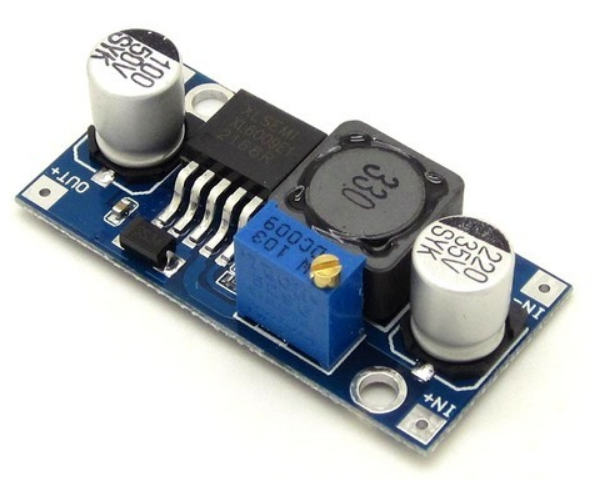
\includegraphics[width=0.5\linewidth]{Imagenes/DCDC}
		\end{figure}
	
	\subsection{Entradas}
	
	La etapa de entradas mostrada en la Figura \ref{fig:BEntradas} está enfocada principalmente a sensores y circuitos que permitan conocer el estado del entorno, es decir, que permitan medir magnitudes como temperatura, iluminación, movimiento, presencia de lluvia, calidad de aire, entre otras. Esta etapa también permite sincronizar el dispositivo con la red eléctrica a la cual se encuentra conectado. Toda esta información tiene como destino la unidad central de mando para vincularla con el resto del sistema IoT.
	
	\begin{figure}[H]
		\centering
		\caption[Etapa de Entradas.]{Etapa de Entradas. [Imagen Propia]}
		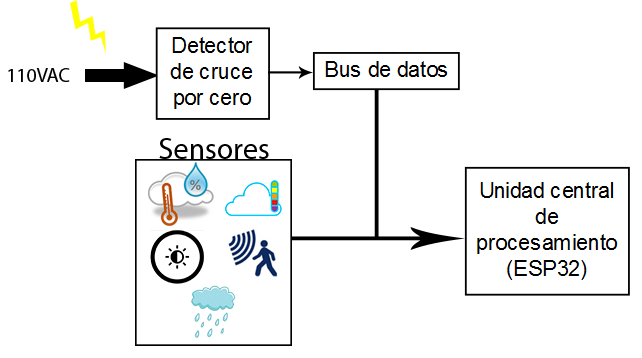
\includegraphics[width=0.7\linewidth]{Imagenes/B_Entradas}\label{fig:BEntradas}
	\end{figure}
	
	\paragraph{Sensores:}
		El prototipo viene equipado con una etapa de adquisición de datos con capacidad entre 7 a 134 sensores, pues posee una entrada I2C, ampliando el número de dispositivos conectados, lo cual también permitiría adicionar tareas más específicas en escenarios que lo requieran.\\
		
		Con la finalidad de realizar pruebas del prototipo, se hacen uso de 5 sensores para medir magnitudes y situaciones en el entorno, tal como calidad del aire, temperatura, humedad, luz visible, movimiento y presencia de lluvia, debido a que estas medidas o estados se encuentran en casi cualquier ambiente. Teniendo en cuenta que el ESP32 funciona en voltajes lógicos de 3.3V, se tienen 4 entradas de sensores directamente conectados a los pines de la tarjeta, con la capacidad de cambiar el voltaje de alimentación para 3 de ellos, como se muestra en la Figura \ref{fig:SVS}, pues en el mercado se encuentran sensores que manejan voltajes de alimentación ya sea de 3.3V o 5V, mientras que la cuarta entrada se encuentra alimentada con 5V, ya que tiene un uso específico en las pruebas para el sensor de calidad de aire, esta viene acondicionada con un diodo zener en contraposición, para evitar que la tarjeta ESP32 tenga un voltaje de entrada superior a 3.3V, según se observa en la Figura \ref{fig:S1Aire}.\\
		
		Las tres entradas para sensores de estado (ST1, ST2, ST3), a diferencia de las demás, se encuentran conectadas a pines de la tarjeta que no presentan resistencia de pull down por software, por ello se agregan estas al sistema, tal como se observa en la Figura \ref{fig:ST}.\\
		
		\begin{figure}[H]
			\centering
			\caption[Entrada de sensores.]{Entrada de sensores. [Imagen Propia]}
			\label{fig:SVS}
			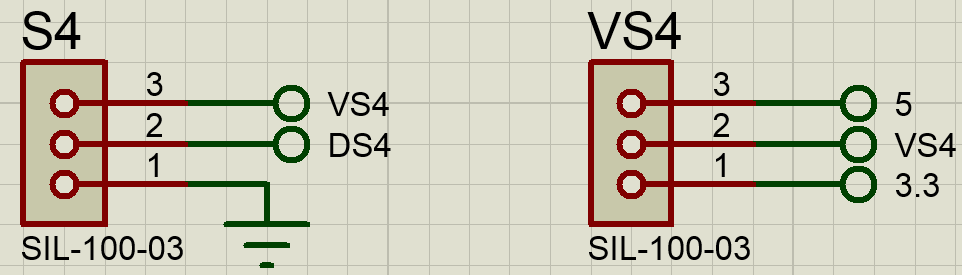
\includegraphics[width=0.7\linewidth]{Imagenes/SVS}
		\end{figure}
	
		\begin{figure}[H]
			\centering
			\caption[Entrada para sensor de calidad de aire.]{Entrada para sensor de calidad de aire. [Imagen Propia]}
			\label{fig:S1Aire}
			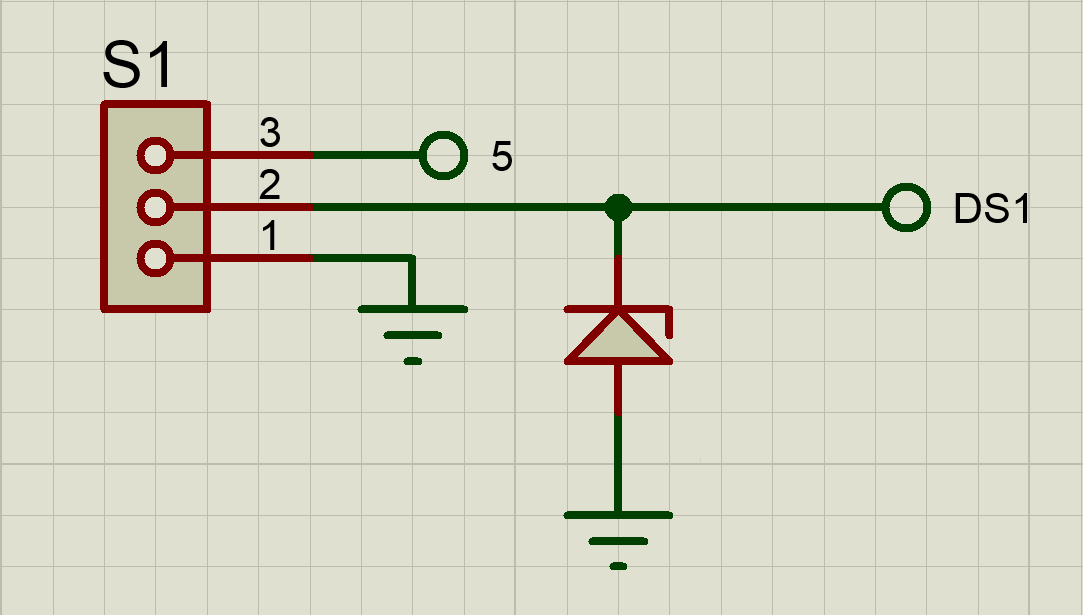
\includegraphics[width=0.6\linewidth]{Imagenes/S1Aire}
		\end{figure}
	
		\begin{figure}[H]
			\centering
			\caption[Entrada para sensores con resistencia de pull down.]{Entrada para sensores con resistencia de pull down. [Imagen Propia]}
			\label{fig:ST}
			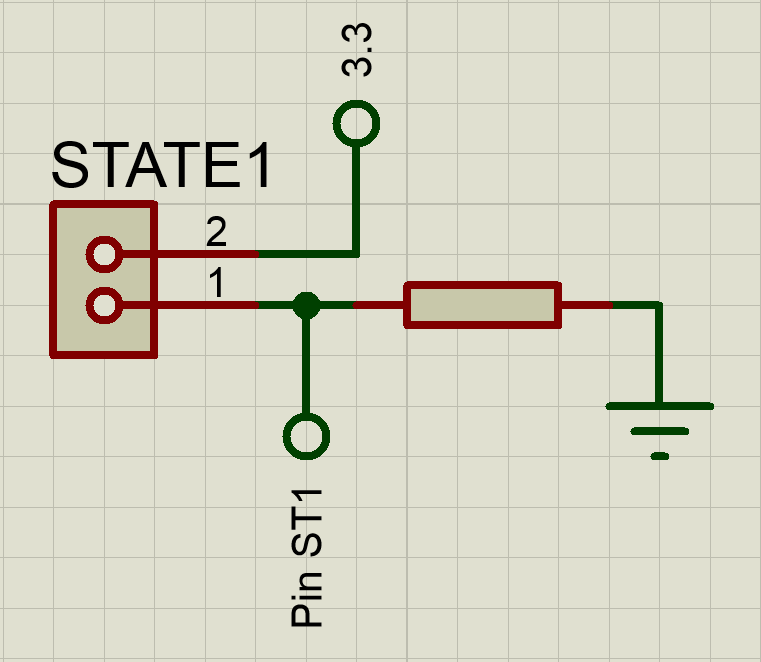
\includegraphics[width=0.5\linewidth]{Imagenes/ST}
		\end{figure}		
	
	
	
	\paragraph{Calibración de audio:}
		Para calibrar la salida audible se hace uso de una resistencia variable (Potenciómetro), el cual permite regular el voltaje de entrada al circuito de amplificación mostrado en la Figura \ref{fig:AUD}; este será descrito en el presente capitulo en la sección de salidas del hardware.
		
	\paragraph{Botón enable:}
		Presionando el botón enable se reinicia la tarjeta ESP32, junto con su firmware.
		
	\paragraph{Botón reset:}
		Presionando el botón reset se borran las credenciales ingresadas para la conexión del ESP32 a la red WiFi.\\
		
	\subsection{Salidas}
	
	Las salidas del prototipo están vinculadas directamente con el circuito de control correspondiente a las cargas, es decir, las salidas DC están diseñadas para ser controladas por medio de PWM, mientras que las salidas AC por medio de control por Angulo de fase en sus salidas controladas. Estos circuitos de contorl están manejados por la unidad central de mando tal como se observa en el esquema de esta etapa ilustrado en la Figura \ref{fig:BSalidas}.\\ 
	
	\begin{figure}[H]
		\centering
		\caption[Etapa de Salidas.]{Etapa de Salidas. [Imagen Propia]}
		\label{fig:BSalidas}
		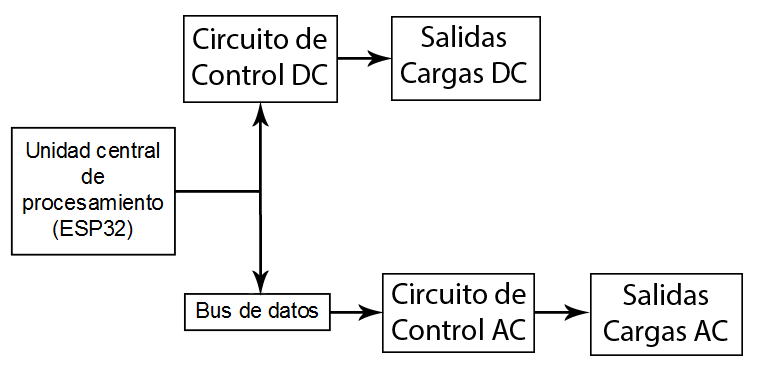
\includegraphics[width=0.7\linewidth]{Imagenes/B_Salidas}
	\end{figure}	
	
	\paragraph{Etapa de potencia AC:}
		Se encuentra diseñada a una potencia de 2000W en un total de seis cargas, cuatro de ellas cuentan con un circuito para el control por ángulo de fase, como se observa en la Figura \ref{fig:CAC1}, con una capacidad individual de 500W, gracias a el TRIAC BTA26600, el cual soporta una corriente máxima de 25A. Con el fin de proteger el ESP32, se hace uso de optoacopladores MOC3021, debido a su funcionalidad para aislar circuitos de forma óptica.\\
		
		\begin{figure}[H]
			\centering
			\caption[Control por ángulo de fase.]{Control por ángulo de fase.  [Imagen Propia]}
			\label{fig:CAC1}
			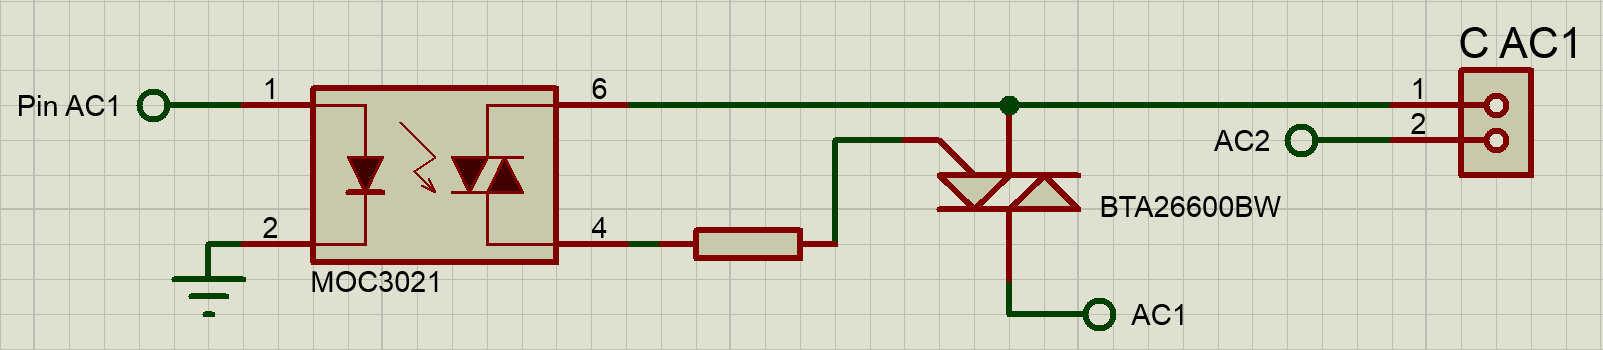
\includegraphics[width=0.8\linewidth]{Imagenes/CAC1}
		\end{figure}
	
		Las dos cargas restantes corresponden a un sistema de encendido y apagado, cuyo funcionamiento se basa en un relevador SRA-05VDC-CL ya que permite una activación a 5V, realizada a través de un transistor BJT como switch, gracias a este relé, las salidas tienen capacidad de hasta 200W cada una. En la Figura \ref{fig:ONOFAC} se observa el circuito diseñado en Proteus. Para proteger el ESP32, el prototipo se vale de ese dispositivo, puesto que presenta un aislamiento magnético por la naturaleza de su operación.\\
	
		\begin{figure}[H]
			\centering
			\caption[Interruptor para cargas AC.]{Interruptor para cargas AC.  [Imagen Propia]}
			\label{fig:ONOFAC}
			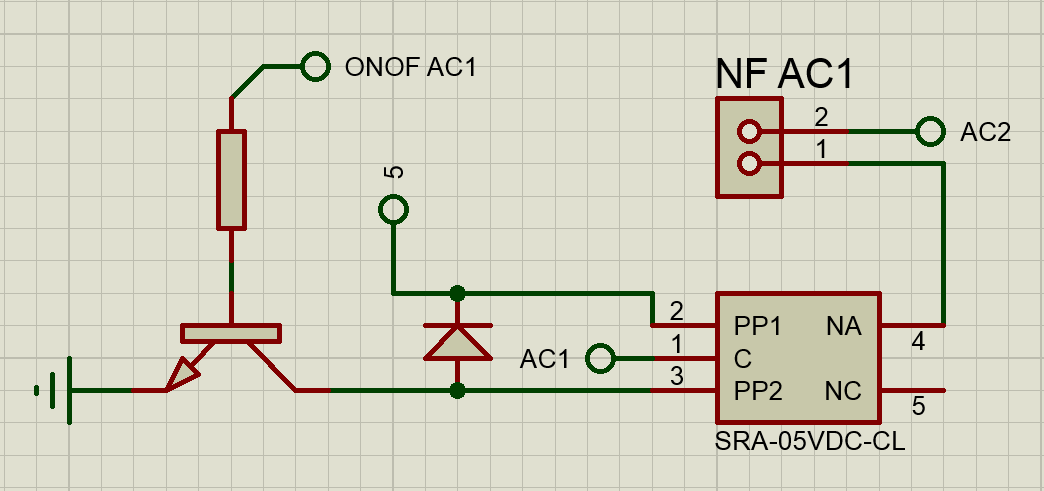
\includegraphics[width=0.7\linewidth]{Imagenes/ONOFAC}
		\end{figure}
	
		Dentro de la etapa AC se encuentra el detector de cruce por cero, el cual cuenta con un fototransistor 4N25, debido a su alta capacidad de aislamiento, tomando la onda rectificada completa y pasándola a un nivel lógico de 3.3V, esta parte del circuito se observa en la Figura \ref{fig:DC01}; para que la señal sea más confiable se hace uso de un Schmitt-Trigger CD40106 mostrado en la Figura \ref{fig:DC02}, valiéndose de la histéresis de voltaje garantizando que la señal de salida sea poco susceptible al ruido \cite{DC0}.\\
		
		\begin{figure}[H]
			\centering
			\caption[Detector de cruce por cero.]{Detector de cruce por cero.  [Imagen Propia]}
			\label{fig:DC01}
			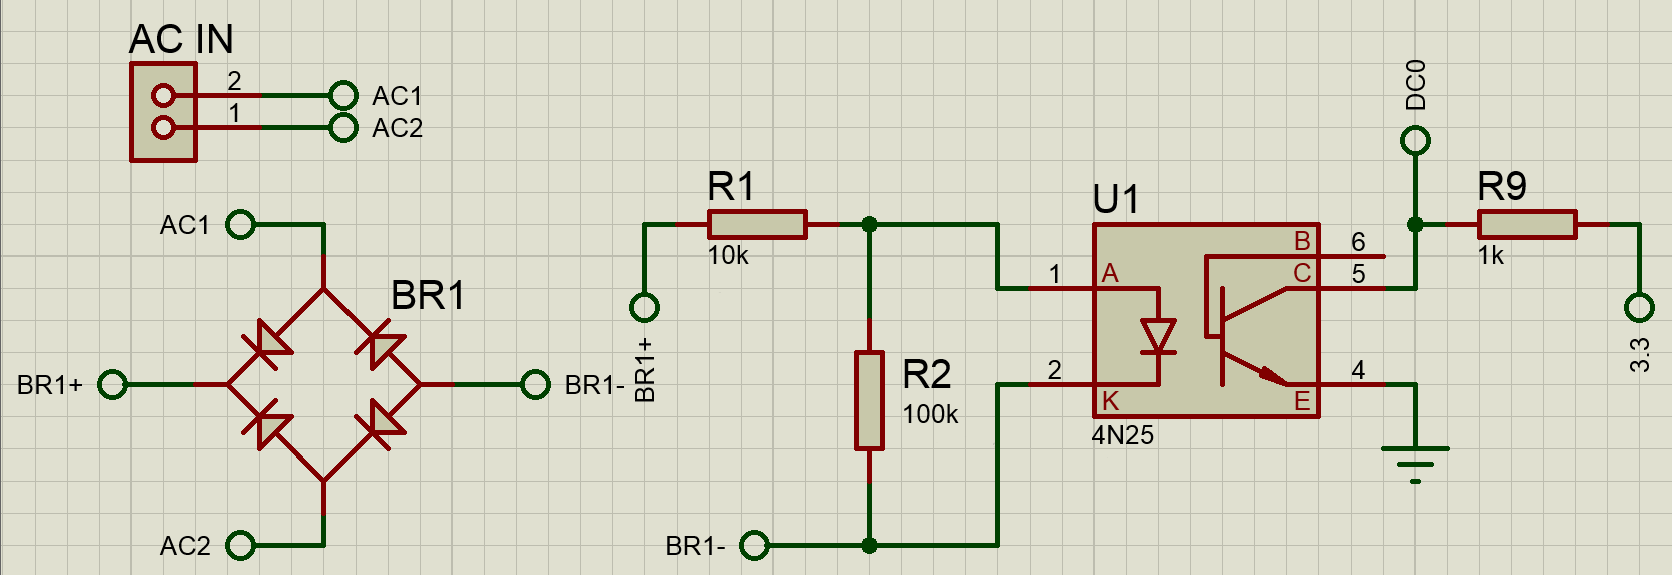
\includegraphics[width=0.85\linewidth]{Imagenes/DC01}
		\end{figure}
	
		\begin{figure}[H]
			\centering
			\caption[Schmitt trigger para el detector de cruce por cero.]{Schmitt trigger para el detector de cruce por cero. [Imagen Propia]}
			\label{fig:DC02}
			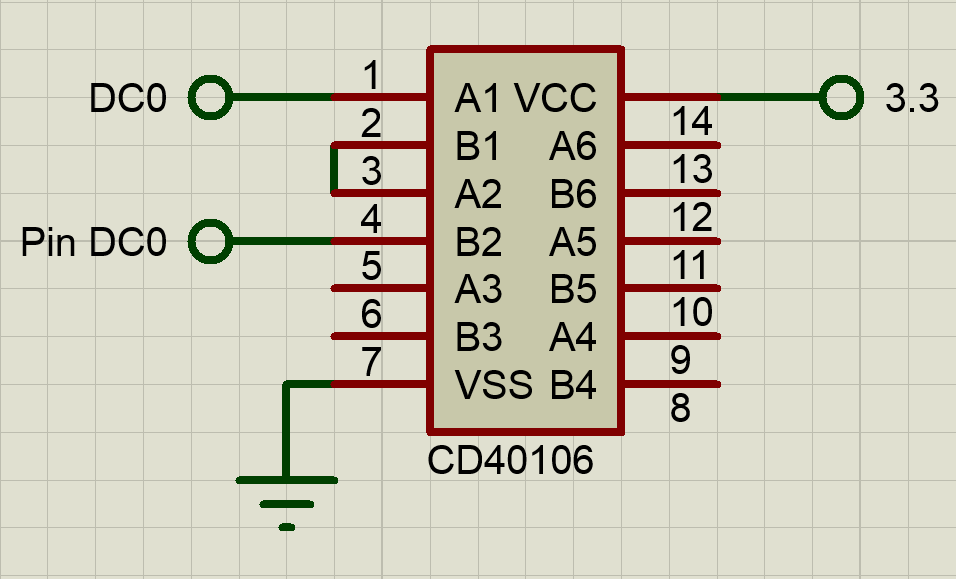
\includegraphics[width=0.5\linewidth]{Imagenes/DC02}
		\end{figure}
	
	\paragraph{Etapa DC:}
		Esta etapa cuenta con cuatro salidas de control diseñadas para cargas de 12V, de las cuales, dos de ellas tienen un enfoque a motores, puesto que está equipada con control de velocidad a base de PWM e inversión de giro con un puente H usando transistores mosfet IRLZ44N; los cuales fueron seleccionados debido a que permiten ser activados a niveles lógicos, además de su capacidad para trabajar en potencias de hasta 50W. El puente h se encuentra controlado por un circuito integrado L293D, que garantiza un voltaje Vgs adecuado para la correcta activación del los transistores; este circuito se muestra en las Figuras \ref{fig:L293D} y \ref{fig:CDC}.\cite{IRL}.\\
		
		Las dos salidas restantes también cuentan con mosfet IRLZ44N, y su control igualmente es a base de PWM, mas no permite realizar la inversión de giro, por lo cual se enfoca a dispositivos como lámparas LEDs. El diseño en Proteus se muestra en la Figura \ref{fig:ONOFDC}.\\
		
		\begin{figure}[H]
			\centering
			\caption[Integrado L293D.]{Integrado L293D. [Imagen Propia]}
			\label{fig:L293D}
			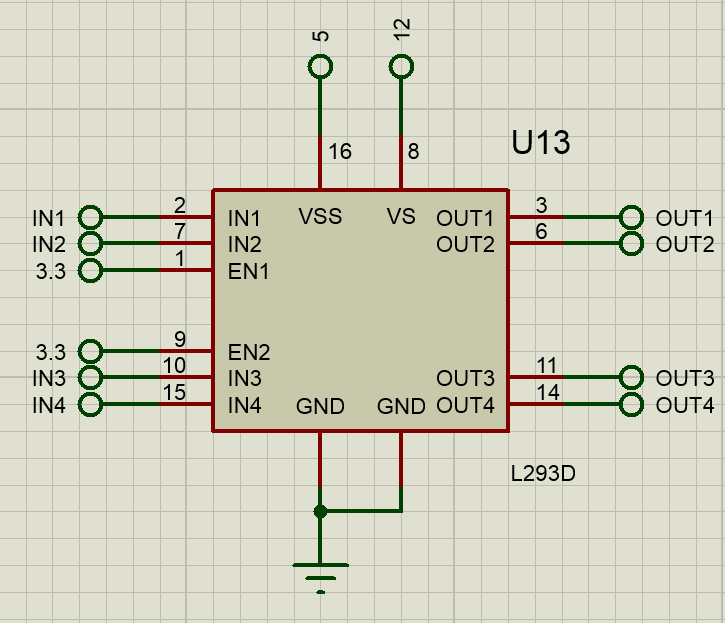
\includegraphics[width=0.5\linewidth]{Imagenes/L293D}
		\end{figure}
		
		\begin{figure}[H]
			\centering
			\caption[Puente H para control de motores DC.]{Puente H para control de motores DC. [Imagen Propia]}
			\label{fig:CDC}
			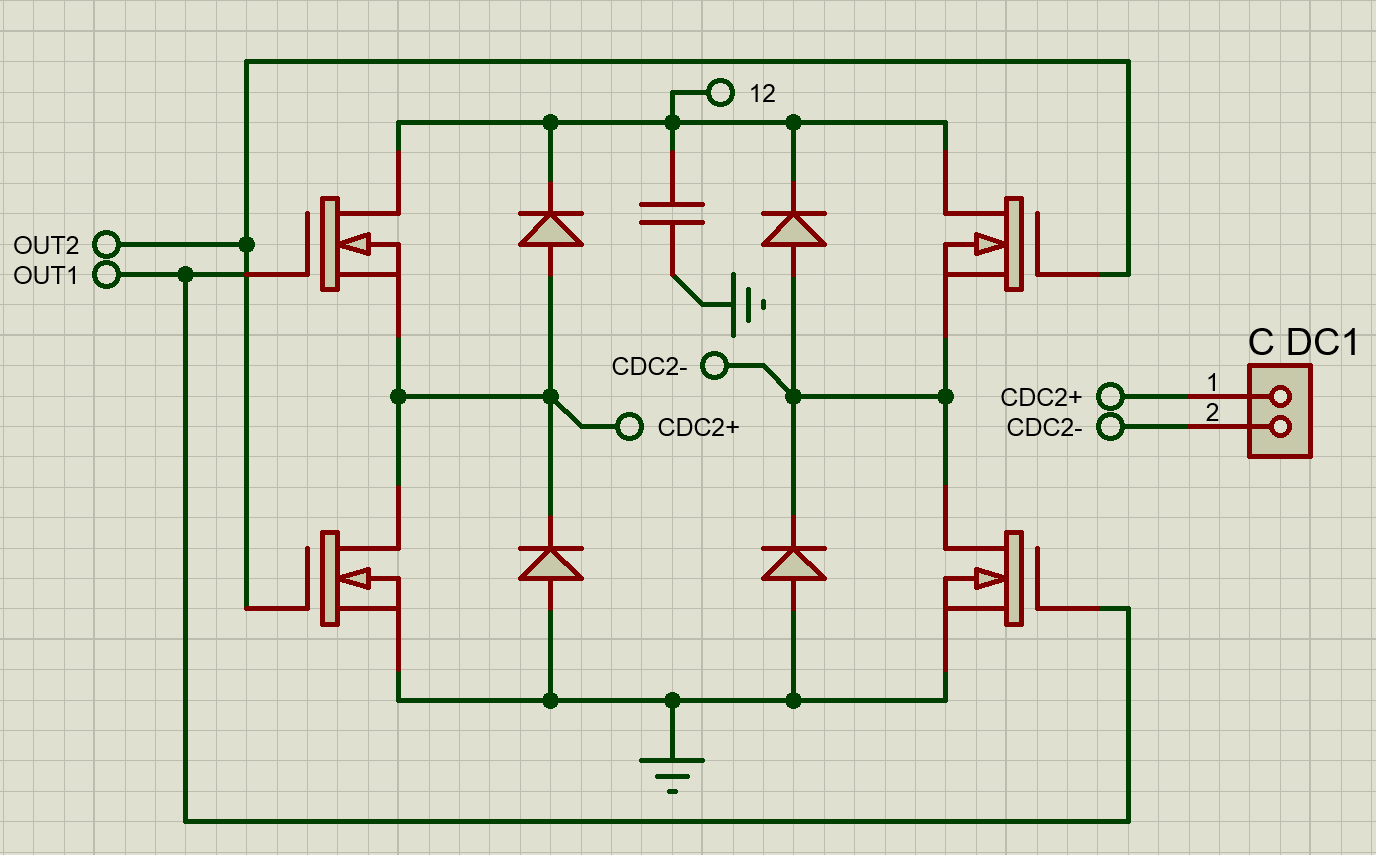
\includegraphics[width=0.7\linewidth]{Imagenes/CDC}
		\end{figure}
	
		\begin{figure}[H]
			\centering
			\caption[Control para cargas DC.]{Control para cargas DC. [Imagen Propia]}
			\label{fig:ONOFDC}
			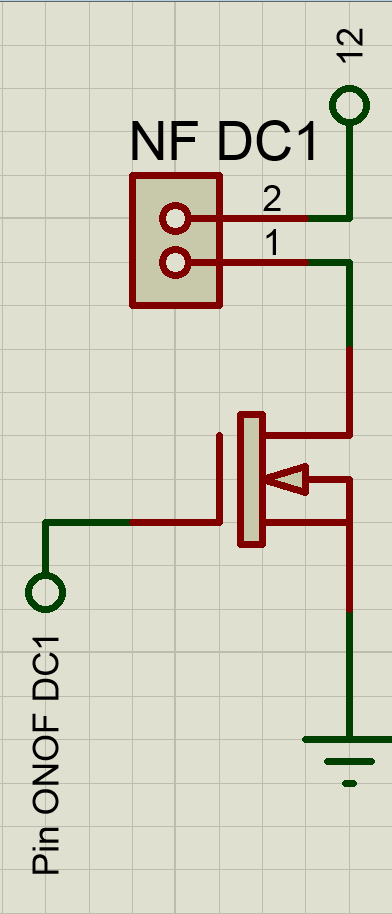
\includegraphics[width=0.15\linewidth]{Imagenes/ONOFDC}
		\end{figure}
	
	\paragraph{Salida audible:}
		Está diseñada para emitir sonidos a una sola frecuencia, o sonido mono estéreo, caso dado cuando se activa una regla programada en la aplicación web, enfocada a las cargas de encendido y apagado, tanto de la etapa de potencia AC como la etapa DC; el sonido emitido por el prototipo corresponde a una voz con tonalidad femenina, pronunciando el estado en el cual se configura la carga según la regla (ya sea encendido, o apagado).\\
		
		El circuito utilizado para la salida audible está basado en el amplificador de audio LM386, implementando el esquema típico de aplicación ilustrado en su datasheet \cite{LM386}. En la Figura \ref{fig:AUD} se observa implementado en el software Proteus.\\
		
		Como se mencionó anteriormente, el circuito presenta un potenciómetro a la entrada para calibrar el voltaje de esta, con el objetivo de no saturarla y que la salida sea lo más fiel posible.\\
		
		\begin{figure}[H]
			\centering
			\caption[Circuito típico para el LM386.]{Circuito típico para el LM386.  [Imagen Propia]}
			\label{fig:AUD}
			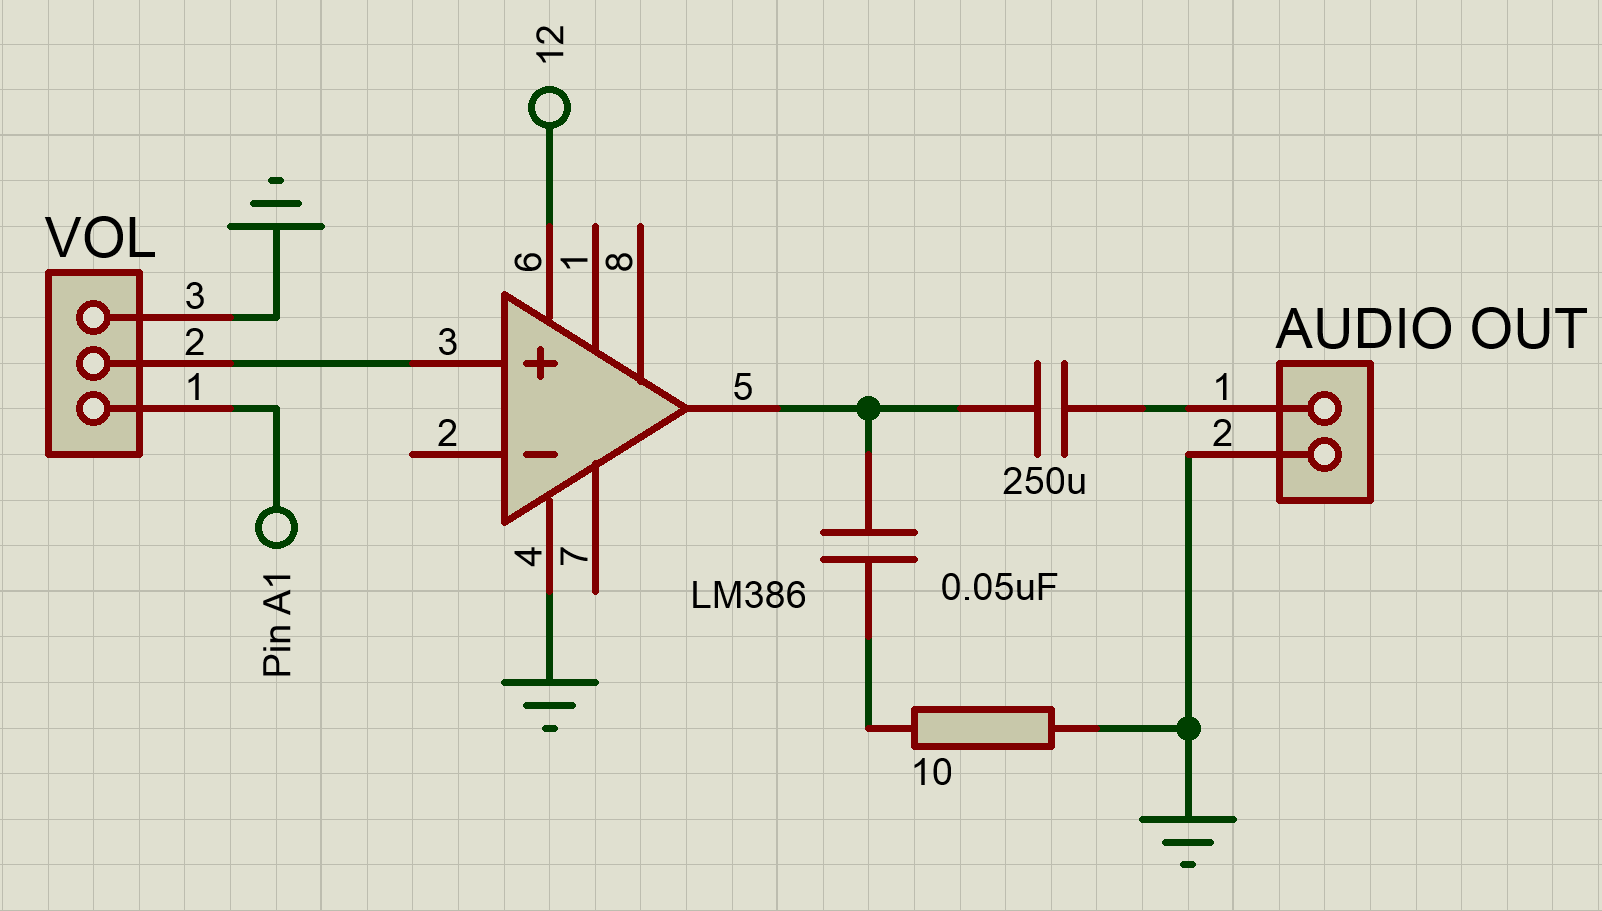
\includegraphics[width=0.7\linewidth]{Imagenes/AUD}
		\end{figure}		
				
\section{Software}

\subsection{Aplicación Sistema Embebido}
La aplicación se desarrolla sobre el framework o SDK oficial de Espressif Systems ESP-IDF, el cual posee una documentación \cite{ES} muy útil a la hora de utilizar las diferentes APIs presentes en este; para el desarrollo es necesario contar con los requisitos que se observan en la Figura \ref{fig:what-you-need}. Esta característica del sistema incluye un kernel de tiempo real llamado FreeRTOS, el cual da soporte al manejo de los diversos recursos del sistema; al ser un RTOS, las funciones se definen mediante tareas, entonces cada funcionalidad de la tarjeta o grupo de funcionalidades se desarrolla en una o varias tareas que realicen las acciones adecuadas. Se usa este framework debido a que es el oficial para este chip, de este modo está en constantes actualizaciones y agregando nuevas funcionalidades.\\

\begin{figure}[H]
	\centering
	\caption[ESP-IDF.]{ESP-IDF. Tomado de: \cite{ES}}
	\label{fig:what-you-need}
	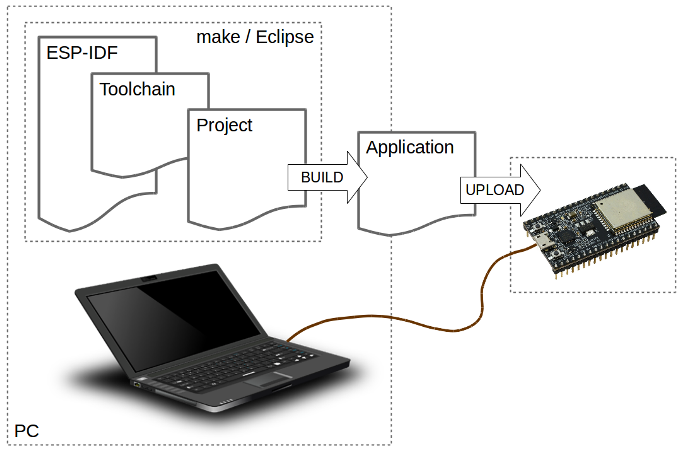
\includegraphics[width=0.5\linewidth]{Imagenes/what-you-need}
\end{figure}

Además, la aplicación a desarrollar se puede observar en la Figura \ref{fig:App}, este diagrama explica, por ejemplo, en el caso de los sensores, cada uno tiene una tarea para la lectura y gestión de datos, así como también ocurre de manera similar con las salidas de la tarjeta, pues cuentan con tareas encargadas de la gestión del encendido y apagado, asimismo para el control de cargas, ya sea por ángulo de fase o PWM. Antes de realizar las funciones de la aplicación se procede a configurar el framework, sus componentes y algunas partes del freeRTOS.\\

\begin{figure}[H]
	\centering
	\caption[Diagrama Aplicación del Sistema Embebido.]{Diagrama Aplicación del Sistema Embebido. [Imagen Propia]}
	\label{fig:App}
	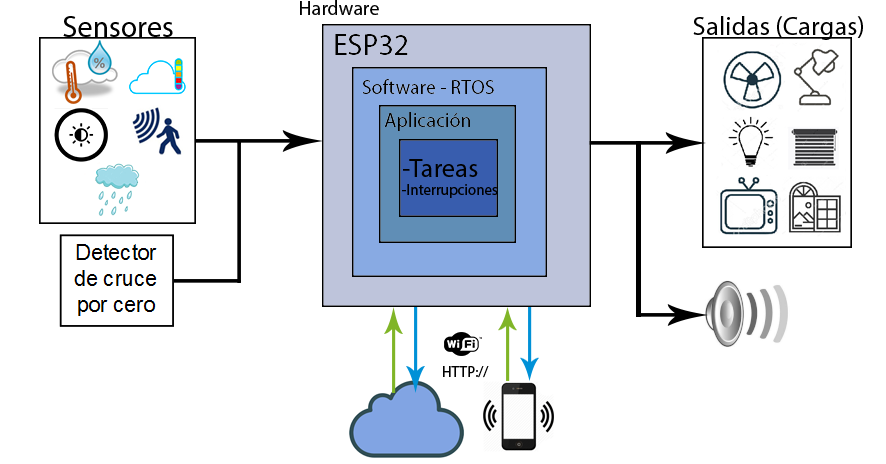
\includegraphics[width=0.7\linewidth]{Imagenes/B_Aplicacion}
\end{figure}

\subsubsection{Configuración ESP-IDF}

El framework usa el sistema Kconfig para facilitar la configuración \cite{ES}, provee una interfaz gráfica sencilla, ilustrada en la Figura \ref{fig:Kconf}, donde se configuran distintos parámetros de este.

\begin{figure}[H]
	\centering
	\caption[Interfaz de Configuración ESP-IDF.]{Interfaz de Configuración ESP-IDF. [Imagen Propia]}
	\label{fig:Kconf}
	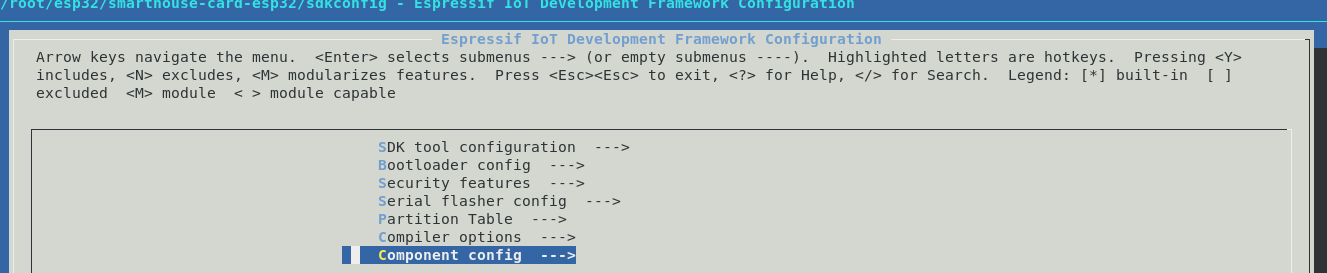
\includegraphics[width=\linewidth]{Imagenes/Kgui}
\end{figure}

Para el desarrollo se modifican ítems en ``Serial Flasher Config'' como el tamaño de la flash a usar, al valor máximo de 4MB, el puerto serial donde se detecta el ESP32 y además la velocidad de transmisión a un valor de 115200 bps. Otro punto que se configura es la tabla de particiones, ya que el ESP32 puede tener una o varias aplicaciones \cite{ES}, en este caso solo contiene una y se usa la tabla de particiones por defecto que provee el framework. Asimismo, en la parte de ``Component Config'' se eligen los componentes que están disponibles y sus configuraciones básicas, por ejemplo, las opciones para el RTOS, donde se configura en qué núcleo se va a ejecutar el sistema operativo, que timer va a usar y también su tick rate, que en este caso es de 100Hz; también se activa el Wi-Fi con la configuración por defecto y que la potencia máxima sea de 20dBm para interfaz física y también se configura una velocidad de la CPU de 240MHz. Esta interfaz permite configurar muchos más componentes que no se usaron o se dejan con la configuración por defecto.\\

%https://docs.espressif.com/projects/esp-idf/en/latest/api-reference/kconfig.html

La implementación de esta aplicación se divide en las entradas, salidas y comunicación, como se puede observar en la Figura \ref{fig:App}. En la parte de entradas se crean tareas o interrupciones encargadas de la lectura de los sensores que previamente están acondicionados por el hardware para su correcto funcionamiento; del mismo modo las salidas cuentan con diferentes tareas para gestionar su estado, es decir, si se encuentran encendidas/apagadas o tienen algún tipo de control y finalmente la parte de comunicaciones se gestiona a través de Wi-Fi para la conexión física, protocolo TCP para la conexión de los datos a través de Internet usando HTTP para encontrar los recursos en la red.

\subsubsection{Entradas}

En esta sección se han desarrollado diferentes tareas o interrupciones para cada uno de los sensores, ya que por su naturaleza sus tiempos de muestreo son distintos, por ejemplo, la temperatura y humedad son variables que tienen cambios lentos en comparación con la luminosidad; por otra parte los sensores de movimiento o lluvia se implementan por medio de interrupciones, ya que por su naturaleza están enfocados a eventos, es decir, si detecto lluvia o hubo movimiento genere una interrupción que envié los datos a la aplicación web. Por este motivo se tienen en cuenta dichas características para crear diferentes tareas que realicen la gestión de cada dispositivo, con diferentes tiempos de muestreo y utilizando distintos métodos para leer sus valores, las tareas creadas se pueden encontrar con más detalle en el Anexo \ref{AnexoA} en la Tabla \ref{table:tasks}.\\

Para el detector de cruce por cero, el sensor de movimiento y el de lluvia se utilizan interrupciones, ya que no es necesario estar monitoreando estas entradas sino que generan una señal para que la aplicación realice alguna acción. La interrupción instalada para el pin del detector de cruce por cero da inicio a dos timers para que se puedan controlar las cargas AC con el control de ángulo de fase, estos son diferentes al que usa el RTOS para su funcionamiento; mientras que la interrupción de los sensores envían datos a una tarea que identifica cual señal está recibiendo y envía la información a una tarea central.\\

En los demás sensores se tienen tareas con diferentes tiempos de espera para su lectura. En el sensor de luminosidad se utiliza una interfaz I2C para su lectura, para esto se instala el driver I2C en los pines 33 y 32 configurando las direcciones del sensor (esclavo) y del ESP32 (maestro); el dispositivo de calidad de aire arroja datos analógicos, por lo tanto se utiliza el driver del ADC para su lectura, instalándolo en el pin correspondiente; el sensor de temperatura y humedad posee una comunicación 1-Wire por lo tanto se envía una trama que pide datos al DHT11 y este responde por el mismo cable, para este sensor fue necesario el desarrollo de una librería con el fin de su correcto funcionamiento, tomando como referencia algunas librerías de arduino y otros encontradas en la web para su uso.\\

\subsubsection{Salidas}

En cuanto a las salidas se tienen dos grupos, las salidas DC y las salidas AC. En las salidas DC se tiene inversión de giro y control de velocidad para motores, estás son dos de las cuatro salidas, para realizar este control sobre los motores DC se instala el driver de la librería LedC el cual genera señales de PWM en los pines donde se instale y se encuentra en el ESP-IDF, asimismo en las otras dos se cuenta con este driver pero solo cuenta con el control de energía entregada más no con el de inversión de giro. \\

Las salidas AC tienen control de potencia por ángulo de fase, para asegurar este control se utiliza el detector de cruce por cero y los timers que activa con cada interrupción, con el propósito de activar el switch en algún punto de un semiciclo de la onda AC, además cuenta con dos salidas de on/off, las cuales usan pines GPIO.\\

Las salidas de AC controladas tienen una tarea dedicas a ellas igualmente que las salidas para motores DC. Las salidas DC con un control simple y las salidas AC on/off se encuentran en una misma tarea y tienen la posibilidad de activarse por reglas de tiempo programadas desde la aplicación web, es decir, que se encienda o se apague a una hora determinada por el usuario. Esta regla también activa una tarea de audio, la cual por medio de un pin usado como DAC y utilizando el driver I2S reproduce ciertos audios precargados en la aplicación. Cabe resaltar que todas estas tareas reciben la información de una tarea central, cada una procesa los datos que le pertenecen y realiza acciones basándose en estos.\\

\subsubsection{Comunicación}

En la aplicación se dan diferentes tres tipos de comunicación, dos de carácter interno (dentro de la misma solución) y dos externas a través de Wi-Fi. Las comunicaciones internas se dan entre las tareas de entradas y una tarea central y entre esta y las tareas de salida.\\

Para las tareas internas se usan colas, ya que es la forma más común comunicación entre tareas en un sistema operativo, así que hay una cola para las entradas y otra para las salidas, estas colas las gestiona la tarea ``http\_get\_task'', recibiendo los datos de lectura de los sensores, como se observa en la Figura \ref{fig:colas} y enviando los datos para las salidas de la tarjeta. El tipo de variable que manejan estas colas son strings organizados en formato JSON.\\

\begin{figure}[H]
	\centering
	\caption[Comunicación por colas.]{Comunicación por colas. [Imagen Propia]}
	\label{fig:colas}
	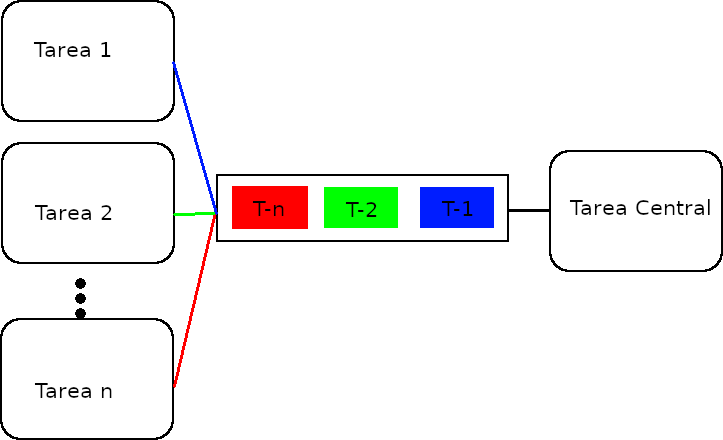
\includegraphics[width=0.5\linewidth]{Imagenes/B_colas}
\end{figure}

Las tareas externas se componen en dos pero no funcionan en paralelo, es decir, si está activa una de estas la otra está inactiva. Este modo de funcionamiento se debe a que una tarea permite que el usuario a través de Wi-Fi para el acceso a la red, IPv4, TCP como protocolo de transporte y un servidor local HTTP en el ESP32 se puedan ingresar las credenciales para la red Wi-Fi a la que se conecta la tarjeta para su salida a Internet. La otra tarea se ha mencionado anteriormente como tarea central, la cual después de verificar la conexión a Internet, conectándose por medio de Wi-Fi al módem o enrutador, comienza a gestionar la escritura y lectura de datos de la aplicación web por medio del protocolo HTTP; leyendo y enviando datos en el sistema embebido, una librería muy útil en este intercambio de datos es cJSON que permite la comprensión del texto en estructura JSON, además de las otras encargadas de gestionar toda la conexión con la aplicación web, como LwIP.\\
%Sobre el firmware se desarrollan los siguientes temas:

%\paragraph{Tareas:}Se ejecutan constantemente en el sistema operativo, realizando diferentes funciones para lectura, escritura y control.

%\paragraph{GPIO:}El ESP-WROOM-32 posee diferentes GPIO, los cuales se usan para leer o escribir señales digitales; en cuanto a los sensores, se pueden enviar señales con el fin de iniciar su lectura o simplemente tener el pin en modo entrada y leerlo cada cierto intervalo de tiempo generando datos de lectura, o en modo salida para el control de los diversos dispositivos que se han desarrollado en el hardware.

%\paragraph{ADC,DAC:}Los ADC se usan para leer los datos de algunos sensores que proporcionan señales analógicos, por este motivo se hace la conversión de la señal analógica a un valor digital dentro de la tarjeta, así luego identificar el dato de la lectura del sensor. Los DAC son usados para realizar la operación contraria, es decir, teniendo valores digitales convertirlos a un valor analógico por ejemplo generar audios o diferentes señales a partir del software. Para esto se usa el driver correspondiente que provee el ESP-IDF para cada funcionalidad, sea para ADC o DAC o para salidas de audio por medio de I2S.

%\paragraph{Consola:}para realizar diferentes pruebas directamente desde la tarjeta, se usa la opción de la consola, la cual se comunica por medio del puerto serie, para esto se crean las funciones y los comandos que estaran disponibles; algunos son \textit{http}, para ejecutar las peticiones http manualmente y observar su respuesta, \textit{pin} para realizar la prueba de un pin digital como entrada o salida, \textit{help} para observar la lista de comandos, entre otros.

%\paragraph{HTTP Request:}Las peticiones HTTP son indispensables en estas aplicaciones del campo IOT, por tal motivo en el desarrollo del firmware se usan las librerías pertinentes para realizarlas como LwIP que se encarga de la gestión del protocolo TCP/IP, cJSON para la gestión de los datos recibidos del servidor. Asimismo leer las respuestas de estas peticiones desde el servidor, ya que por medio de dichas peticiones se encuentra la comunicación tarjeta-servidor.

%\paragraph{Servidor HTTP Local:}El servidor local se desarrolla para proporcionar las credenciales de la red WiFi a la cual se debe conectar la tarjeta, para este servidor se adicionan las paginas en HTML y las librerías de JavaScript y hojas de estilo para su visualización por medio de diferentes APIs de la librería LwIP y hace uso de algunas peticiones HTTP como GET y POST para garantizar el correcto funcionamiento. La tarjeta solo puede gestionar máximo 4 hosts conectados al mismo tiempo.

%\paragraph{Hora de Red:}Se obtiene la hora mediante el protocolo simple de tiempo de red (SNTP), este resulta de gran utilidad para la sincronización de los relojes de los sistemas informáticos. Se mantiene actualizada con el objetivo de realizar diferentes acciones respecto a esta. Además, se usan librerías propias de un sistema operativo como time, sys para almacenar y acceder a dicho dato luego de la sincronización con la hora de la red.

%\paragraph{Timers:}La tarjeta posee dos grupos de timers y cada uno tiene dos timers, un timer lo usa el sistema operativo, otro es configurado con el fin de realizar el control de potencia AC por ángulo de fase, para tener la sincronía necesaria con la señal de la red eléctrica.

%\paragraph{I2C:}El protocolo I2C se activa por medio de la instalación del driver en algún par de pines GPIO disponibles en la tarjeta. Se configura e inicia y posteriormente se crea una tarea la cuál se encarga de solicitar y leer los datos de los diferentes sensores conectados a este.

%\paragraph{PWM:}Se ha mencionado anteriormente que con el propósito de controlar las cargas DC se usa una salida PWM, el ESP32 proporciona esta funcionalidad en algunos de sus pines, para su uso se configura y asignan los valores de funcionamiento por medio de la librería Ledc, la cual proporciona diferentes características para cada canal de PWM que se usa.

%\paragraph{Interrupciones:}Las interrupciones se usan para no gastar recursos en un monitoreo constante de las entradas, sólo cuando exista un cambio de nivel en la entrada el dispositivo desencadena una serie de instrucciones relacionadas con el tipo de interrupción y diversas funciones creadas para esta, la interrupción se usa por medio de los diferentes pines con este propósito en el hardware. Adicionalmente, se deben iniciar estas interrupciones en ciertos puntos del sistema para que no lo saturen antes de arrancar todas sus funcionalidades.

\subsection{Aplicación Web}

En esta sección se desarrolla una aplicación web, la cual se encarga de ejecutar la gestión entre el usuario y la tarjeta por medio de una interfaz gráfica, dicha aplicación se encuentra en la nube para que este disponible desde cualquier lugar con acceso a Internet, como se observa en la Figura \ref{fig:B_appwD}. Es el intermediario de la comunicación humano-máquina, por este motivo la parte gráfica que se desarrolla es sencilla de usar.\\

\begin{figure}[H]
	\centering
	\caption[Diagrama Aplicación Web.]{Diagrama Aplicación Web. [Imagen Propia]}
	\label{fig:B_appwD}
	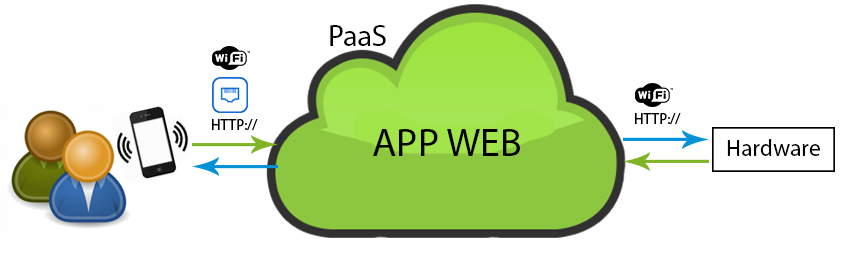
\includegraphics[width=0.7\linewidth]{Imagenes/B_AppWebDllo}
\end{figure}

Se desarrolla la aplicación web de manera local y posteriormente se lanza a un servidor en Internet. Se encuentra compuesta por los siguientes sitios y las diferentes interacciones basadas en las funciones básicas crear, leer, actualizar y borrar (CRUD).\\

\begin{itemize}
	\item Parte Pública
	\item Parte Privada
	\begin{itemize}
		\item Intercambio de datos5
		\item Panel de Control
		\begin{itemize}
			\item Crear
			\item Ver
			\item Editar
			\item Eliminar 
		\end{itemize}
	\end{itemize}
\end{itemize}

De acuerdo con la lista anterior, se toman en cuenta dos partes, una pública y una privada, como se observa en la Figura \ref{fig:index}. De este modo, se usa un patrón de arquitectura Modelo-Vista-Controlador (MVC), siendo este realmente útil ya que separa la lógica de negocio de la interfaz de usuario, incrementando la reutilización y flexibilidad, además de la escalabilidad de ambos aspectos por separado, dicho esto, la aplicación cuenta con diferentes modelos, controladores y vistas \cite{MVC1}. Además, se usa el framework Laravel para desarrollar toda la lógica y las vistas. La lógica está basada en MVC como se menciona, desarrollándolo sobre PHP que es el lenguaje de programación que usa Laravel y la interfaz gráfica se desarrolla con ayuda de HTML5, Bootstrap y JavaScript, como se observa en la figura \ref{fig:B_appweb}, que están integrados en Laravel, para el almacenamiento de datos se usa PostgreSQL el cual lo provee Heroku.\\

Usar la arquitectura MVC y el framework Laravel es muy útil, ya que con las funcionalidades que se han provisto es necesario tener un control como el que brinda el MVC y con Laravel crear esta lógica es más sencillo que empezar desde cero, ya que no hay que preocuparse mucho sobre el motor de base de datos porque con el ORM simplemente se realizan las peticiones en PHP y ya el lo traduce a la consulta adecuada. De acuerdo a estas partes propuestas se desarrollan diferentes modelos, controladores y vistas. Los modelos creados se consignan en la Tabla \ref{table:models}, como se ha mencionado los modelos se encargan de interacción entre el controlador y la base de datos.\\

\begin{table}[H]
	\begin{center}
		\caption{Modelos de la aplicación web.}
		\label{table:models}
		\begin{tabular}{|c|p{7cm}|}
			\hline 
			\textbf{Modelo} & \textbf{Descripción} \\ 
			\hline 
			User & Es el encargado de gestionar la información de los usuarios en la aplicación web y base de datos.\\ 
			\hline 
			House & Es el encargado de gestionar la información de las casas de los usuarios en la aplicación web y base de datos.\\ 
			\hline 
			Room & Es el encargado de gestionar la información de las habitaciones de los usuarios en la aplicación web y base de datos.\\ 
			\hline 
			Device & Es el encargado de gestionar la información de los dispositivos de una habitación en la aplicación web y base de datos.\\
			\hline
		\end{tabular} 
	\end{center}
\end{table}

La lista a continuación hace referencia a los controladores desarrollados, cada controlador se encarga de gestionar el modelo y la vista adecuada de acuerdo a la petición del usuario. En cuanto a los controladores User, House, Room, Device todos cuentan con las funciones básica CRUD y presentan las diferentes vistas de cada función con los datos necesarios para cada interacción y se encuentran en la parte privada de la aplicación. El controlador Public es el encargado de gestionar la parte pública de la aplicación. Los controladores Rule, Home y Card se encargan de gestionar las reglas de cada dispositivo, el panel de control de la aplicación web y el intercambio de datos con la tarjeta SmartHouse respectivamente.\\

\begin{itemize}
	\item PublicController
	\item UserController
	\item HouseController
	\item RoomController
	\item DeviceController
	\item RuleController
	\item HomeController
	\item CardController
\end{itemize}

En cuanto a la interfaz gráfica o vistas, en la parte pública se encuentra una vista con la información de contacto del fabricante, solicitudes de registro o productos y la cantidad de usuarios que actualmente están registrados en la aplicación, en general el propósito de la parte publica es permitir solicitudes del nuevo usuario o cliente que ha obtenido la tarjeta. En la parte privada se encuentra la interacción de los usuarios sea administrador, dueño de una casa o de una habitación, para controlar y observar sus datos.\\

\begin{figure}[H]
	\centering
	\caption[Aplicación Web Desarrollada.]{Aplicación Web Desarrollada. [Imagen Propia]}
	\label{fig:B_appweb}
	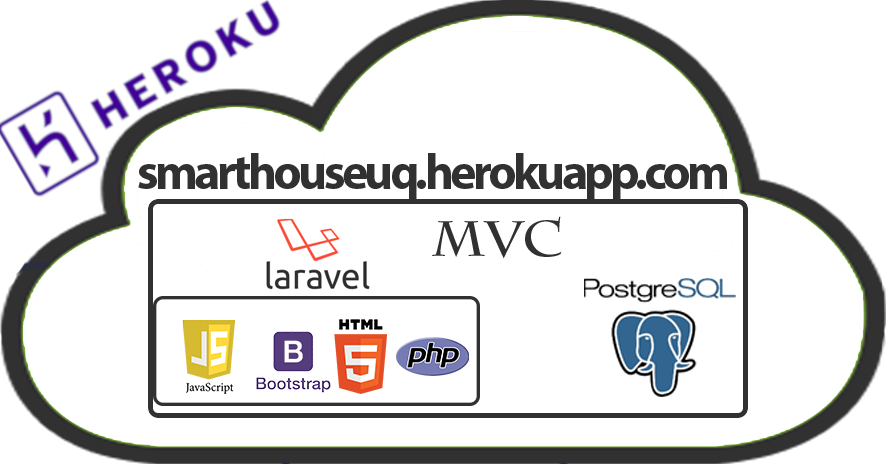
\includegraphics[width=0.5\linewidth]{Imagenes/B_ImplAPPweb}
\end{figure}

Asimismo, por medio de funcionalidades incluidas en el framework como Bootstrap y JavaScript se desarrollan las diferentes vistas que cada usuario posee, así como un panel de control encargado de la gestión de la habitación, las casas y la solución en general. De este modo al usar Bootstrap se tiene un diseño responsivo, lo que permite la correcta visualización de la aplicación web en cualquier tamaño de pantalla y con JavaScript se logra que algunas vista sean interactivas. Las diversas interacciones que tiene cada usuario en el panel de control se garantizan por medio del MVC y el framework, creando diferentes roles para cada tipo de usuario que se esta registrando y realizando la comprobación por parte de los controladores y el middleware que este provee.\\

\begin{figure}[H]
	\centering
	\caption[Página de Inicio.]{Página de Inicio. [Imagen Propia]}
	\label{fig:index}
	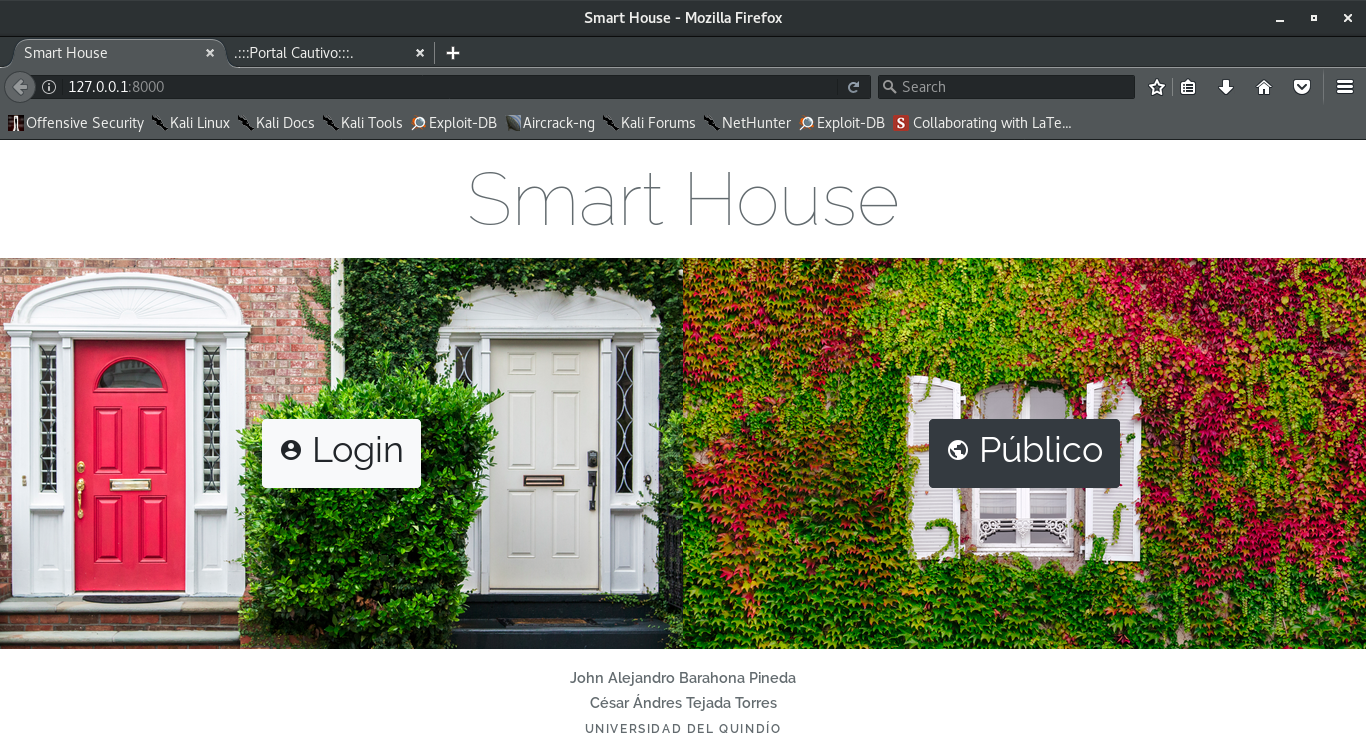
\includegraphics[width=0.5\linewidth]{Imagenes/Index}
\end{figure}

\subsection{Parte Pública}

En esta vista únicamente hay opciones para el contacto y solicitudes, como se menciona anteriormente, es sencilla debido a la poca información que contiene, según se observa en la Figura \ref{fig:publicview}.

\begin{figure}[H]
	\centering
	\caption[Vista Pública.]{Vista Pública. [Imagen Propia]}
	\label{fig:publicview}
	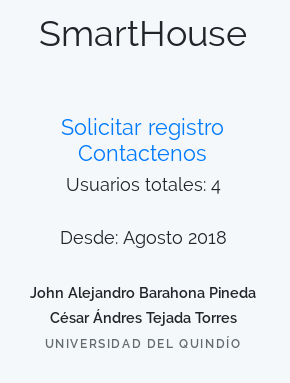
\includegraphics[width=0.25\linewidth]{Imagenes/Public_view}
\end{figure}

\subsection{Parte Privada}

En esta sección es donde se encuentra el Panel de Control para los diferentes usuarios de la aplicación. Se definen tres roles que comprenden los tipos de usuarios de esta solución, un usuario administrador, un usuario casa y un usuario habitación. El usuario administrador es el encargado de gestionar todo en la aplicación, leer, crear, editar y borrar cualquier característica; como los otros usuarios, casas, habitaciones o dispositivos, la vista de este usuario se puede observar en la Figura \ref{fig:views}\textbf{(a)}. El usuario casa se refiere a un administrador de la casa donde se tengan instaladas más de una tarjeta SmartHouse, es decir, que un hogar cuente con tres habitaciones en las cuales todas cuentan con tarjetas de SmartHouse, este usuario tiene la capacidad de leer, editar y controlar las habitaciones de su casa, como se ve en la Figura \ref{fig:views}\textbf{(b)}. Por último el usuario habitación es la mínima unidad, ya que es el cliente que posee una tarjeta SmartHouse instalada en su habitación, este puede gestionar sus dispositivos, leer y editar algunas características propias de su habitación, según se observa en la Figura \ref{fig:views}\textbf{(c)}. En la tabla \ref{table:roles} se puede encontrar un resumen de cada rol.\\

\begin{table}[H]
	\begin{center}
		\caption{Roles en la aplicación web.}
		\label{table:roles}
		\begin{tabular}{|c|p{8cm}|}
			\hline 
			\textbf{Rol} & \textbf{Descripción} \\ 
			\hline 
			Usuario Administrador & Gestiona toda la aplicación web. Puede crear, leer, editar y eliminar diferentes componentes dentro de esta.\\ 
			\hline 
			Usuario Casa & Gestiona su propia casa registrada en la aplicación web. Puede leer y editar características de su propia casa y habitaciones.\\ 
			\hline 
			Usuario Habitación & Gestiona su propia habitación registrada en la aplicación web. Puede leer y editar características de su propia habitación.\\ 
			\hline 
		\end{tabular} 
	\end{center}
\end{table}

Dichos roles se gestionan a través del framework Laravel para asegurar que los propósitos de cada uno se cumplan, cabe resaltar que el usuario administrador no puede gestionar de ningún modo los estados de las salidas que poseen los dispositivos de casa usuario. El desarrollo de estos roles se enfoca en el usuario habitación y el usuario administrador, siendo el usuario casa un ítem adicional para asegurar la escalabilidad de la solución sin tener cambios en la base de datos.\\

%En primera instancia, un usuario administrador, el cual esta encargado de gestionar la aplicación, tiene la posibilidad de crear, ver, editar y eliminar los registros de la aplicación. La vista de este usuario se puede observar en la Figura \ref{fig:views}\textbf{(a)}. Por medio de este se activan las cuentas de los demás, razón por la cual en la parte pública están las opciones de contacto y solicitud de registro.\\

%También existe el usuario dueño de la vivienda donde se encuentra el dispositivo, este es opcional y es para gestionar los dispositivos presentes dentro de un mismo domicilio. Es un administrador de la casa, el cual puede revisar y editar algunos campos de sus usuarios hijos o usuarios habitación y sus diferentes casas y habitaciones registradas a su nombre, como se ve en la Figura \ref{fig:views}\textbf{(b)}, de este modo el rol de dicho usuario es administrar su hogar y visualizar los datos de esta.\\

%Por último, otro rol es el de usuario habitación, el cuál únicamente visualiza sus propios datos, como la habitación y los dispositivos presentes en esta, según se observa en la Figura \ref{fig:views}\textbf{(c)}. A este solo le compete la información de lo que posee en su cuarto, por tal motivo el panel de control muestra una vista general de los datos y el estado de sus dispositivos, además de tener la capacidad de editar partes básicas de su habitación y perfil. Dicho usuario puede o no estar sujeto a un usuario padre o usuario casa, ya que, solamente posee una tarjeta para su habitación y ninguna otra en dicha casa.\\

\begin{figure}[p]
	\centering
	\caption[Vistas de Usuarios.]{Vistas de Usuarios. [Imagen Propia]}
	\label{fig:views}
	\subfigure[Usuario Administrador]{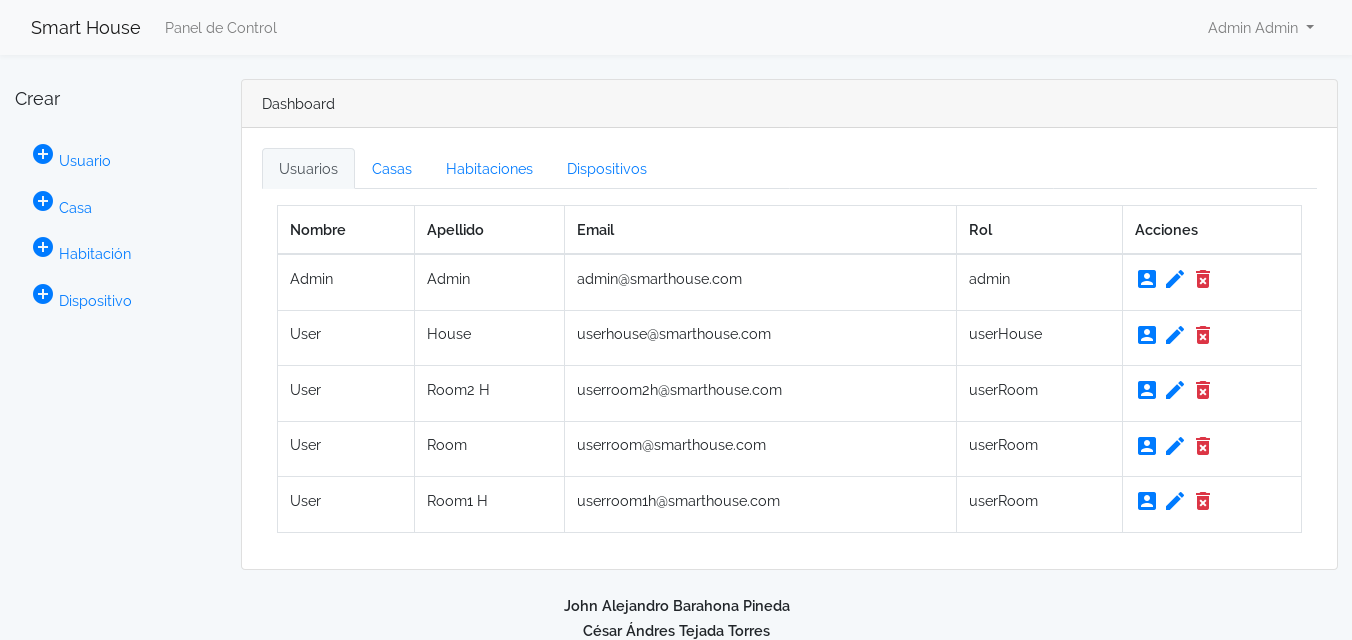
\includegraphics[width=0.9\linewidth]{Imagenes/Admin_view}}
	\subfigure[Usuario de Casa]{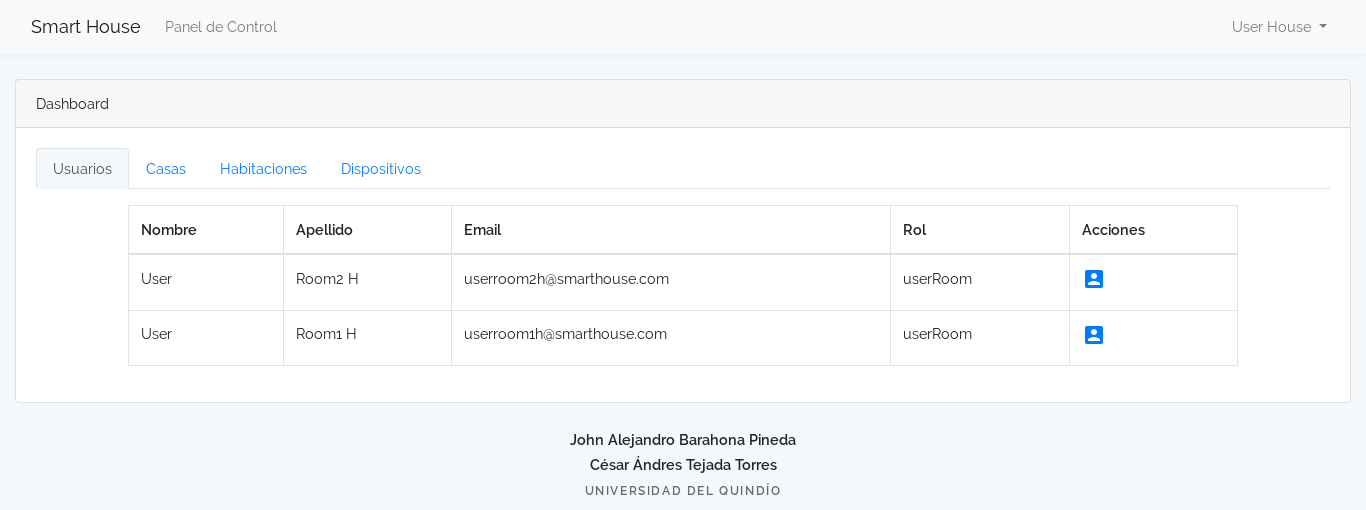
\includegraphics[width=0.9\linewidth]{Imagenes/UserH_view}}
	\subfigure[Usuario de Habitación]{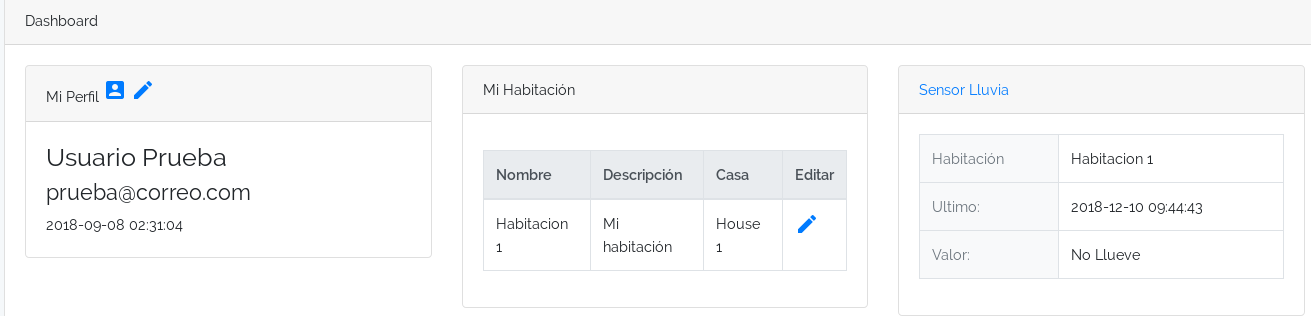
\includegraphics[width=0.9\linewidth]{Imagenes/UserR_view}}
\end{figure}

Además de este panel de control, desde el cuál se realizan las operaciones sobre la aplicación, en la parte privada se encuentra la ruta encargada de la actualización Servidor-Tarjeta, es decir, en esta ruta es donde se intercambia la información. Allí se realiza una petición HTTP tipo GET por parte de la tarjeta, incluyendo en su contenido el id de la habitación en la que está instalada, junto con el token correspondiente a esta, además en la URL se añade un texto tipo JSON en el cual se ubican todas los datos de la lectura actual de los sensores; esta petición la responde el servidor con un texto también tipo JSON que contiene la información pertinente de las cargas o actuadores como se observa la Figura \ref{fig:updateview}. Para dar seguridad a dicha transacción, se utiliza el token mencionado anteriormente, el cual se verifica mediante el id de la habitación comparando el recibido con el almacenado.\\

\begin{figure}[H]
	\centering
	\caption[Página de intercambio de datos.]{Página de intercambio de datos. [Imagen Propia]}
	\label{fig:updateview}
	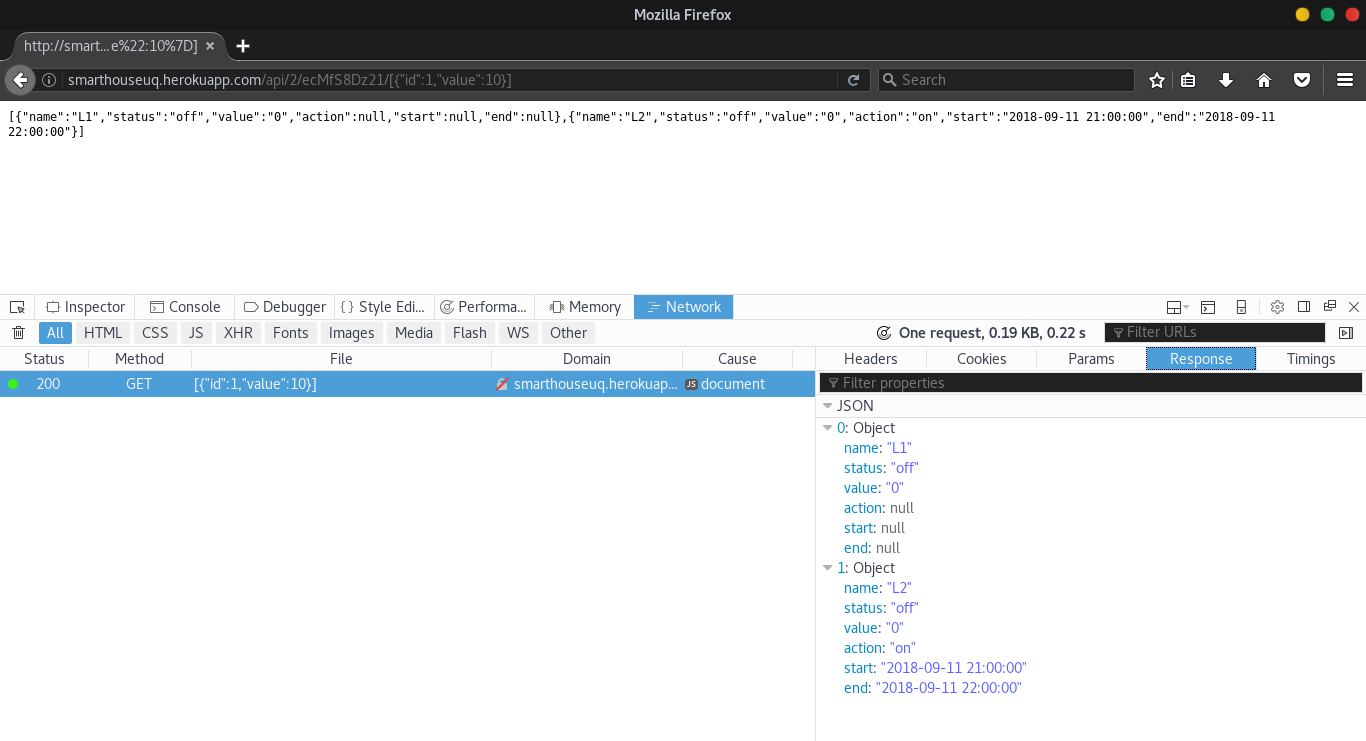
\includegraphics[width=\linewidth]{Imagenes/Update_view}
\end{figure}

Adicional a esto, si el usuario desea añadir, modificar o eliminar una regla, por ejemplo, quiere encender un bombillo led a una hora deseada, esto lo puede lograr mediante el botón de reglas en el panel de control, el cual lo redirige a la vista que se observa en la Figura \ref{fig:rulesview}. En esta se indica una hora de inicio y finalización en la que el bombillo led enciende a la hora de inicio y se apaga a la hora de fin, si es la regla de apagado solo necesita una hora de inicio para apagarlo.\\

\begin{figure}[H]
	\centering
	\caption[Vista para añadir reglas.]{Vista para añadir reglas. [Imagen Propia]}
	\label{fig:rulesview}
	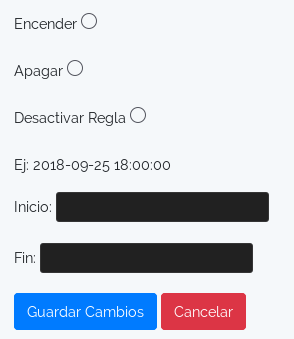
\includegraphics[width=0.25\linewidth]{Imagenes/rules_view}
\end{figure}

%%%%%%%%%%%%%%%%%%%%%%%%%%%%%%%%%%%%%%%%%%%%%%%%%%%%%

%La función de cada parte de esta arquitectura se puede observar en la Figura \ref{fig:mvc}.\\
%
%\begin{figure}[H]
%	\centering
%	\caption[Modelo-Vista-Controlador.]{Modelo-Vista-Controlador. [Imagen Propia]}
%	\label{fig:mvc}
%	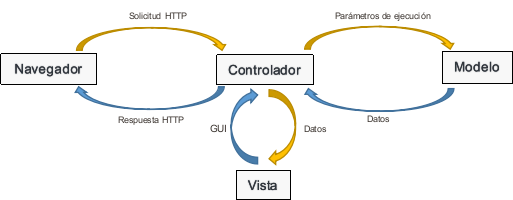
\includegraphics[width=0.7\linewidth]{Imagenes/MVC}
%\end{figure}
%
%
%Su funcionamiento es el siguiente, primero el usuario realiza alguna acción en la interfaz (por ejemplo, presiona un botón, un enlace, etc), luego el controlador recibe (por parte de los objetos de la interfaz-vista) la notificación de la acción solicitada por el usuario. El controlador gestiona el evento que llega, accediendo al modelo y actualizándolo, posiblemente modificándolo de forma adecuada a la acción solicitada por el usuario (por ejemplo, el controlador actualiza los datos del perfil del usuario) y después la interfaz de usuario espera nuevas interacciones del usuario, comenzando el ciclo nuevamente \cite{MVC2}.\\
%
%Este patrón de diseño se usa en la programación orientada a objetos, por lo tanto se realiza la aplicación en el lenguaje de programación PHP, ya que es realmente útil para realizar la gestión de peticiones y envíos de formularios en dicha aplicación, además de que es importante también la gestión de las bases de datos de la aplicación, por este motivo se utiliza un framework basado en este lenguaje y esta arquitectura. Para gestionar las diferentes partes de la aplicación, en este caso se usa el framework Laravel, pues como se menciona anteriormente, está orientado a facilitar las tareas comunes de la mayoría de proyectos web que utilizan HTML5 y PHP.\\

%%%%%%%%%%%%%%%%%%%%%%%%%%%%%%%%%%%%%%%%%%%%%%%%%%%%%%
%
%Además, con este framework se hace uso de un ORM (Mapeo Objeto-Relacional) llamado Eloquent. Esta es una forma de mapear los datos que se encuentran en la base de datos a objetos de PHP y viceversa, esto facilita el uso de diferentes gestores de bases de datos como MySQL, SQLite, entre otras, ya que todas las consultas estan en PHP y el ORM ya se encarga del mapeo a los comandos SQL como se observa en la Figura \ref{fig:orm}. Eloquent usa los modelos para enviar y recibir información de la base de datos\cite{Eloq}.\\
%
%\begin{figure}[H]
%	\centering
%	\caption[ORM]{ORM. [Imagen Propia]}
%	\label{fig:orm}
%	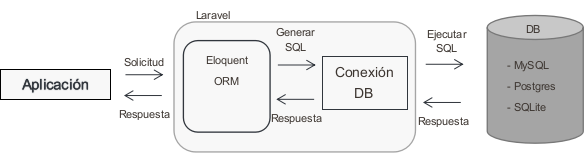
\includegraphics[width=0.7\linewidth]{Imagenes/ORM}
%\end{figure}
%%%%%%%%%%%%%%%%%%%%%%%%%%%%%%%%%%%%%%%%%%%%%%%%%%%%%

\section{Pruebas}

